\chapter{I Asked Miami Millionaires How They Got Rich}

This School of Hard Knocks interview, curated by LazyingArt LLC, gives us almost no formal mathematics on screen, yet it is full of quantitative structure. We are shown outcomes first---a private jet, a Lamborghini, eight-figure exits, a reported annual income near \text{\$}2 million, a business doing \text{\$}5.5 million gross and \text{\$}2.4 million net, and finally a year at \text{\$}752 million in revenue---and only afterward are we allowed to ask what operating rules might generate such outputs. The right way to read the lecture is therefore not as a theorem of wealth, but as a sequence of commercial models: producer versus consumer, gross versus net, speed versus delay, cash flow versus asset stock, and quick richness versus durable freedom.

No validated mathematical frame survives from the video, so every formal relation below is transcript-backed or a cautious reconstruction. We keep close to the narrated order. The lecture begins with spectacle, then moves to classification, then to startup speed, immigrant constraint, accountability, reinvestment, and finally to a higher-scale doctrine of patience, stakeholder balance, and sales.

\section{Opening Montage and the Problem of Method}

The cold open is not yet an explanation. It is an inverse problem. We first see the endpoint and only later search for the mechanism. That is why the opening works: it forces us to ask not whether wealth exists in Miami, but what sorts of decisions, business structures, and time horizons the speakers claim led there.

A few of the reported scales are immediately placed on the table:
\begin{align}
I_{\mathrm{annual}} &\approx \text{\$}2\,\mathrm{M},\\
G &= \text{\$}5.5\,\mathrm{M},\qquad N = \text{\$}2.4\,\mathrm{M},\\
R_{2023} &= \text{\$}752\,\mathrm{M}.
\end{align}
To this we add the more qualitative but still numerical claims of eight-figure exits, tens of millions in yearly earnings, and a city with nearly \(4\times 10^4\) millionaires. The lecture does not prove any of these figures; it uses them to pose the central question. What must a person be doing, structurally, for these scales even to become thinkable?

The host then widens the frame from individual spectacle to a city-level field study. Miami is presented as an environment dense with visible wealth, and the stated purpose is to ask how people became wealthy and how one might begin the path toward financial freedom in 2024. We are now ready for the first real conceptual move.

\section{From Broke to Producer Logic}

The first long interview begins by establishing distance traveled. The speaker has slept in a car, grown up amid scarcity, and later made close to \text{\$}2 million in a single year. But the important turn is not autobiographical. It is classificatory. The lecture wants to divide the social field into economically distinct roles.

\begin{definition}
In the lecture's local vocabulary, a \emph{consumer} is on the side of consuming existing value, while a \emph{producer} is on the side of creating and offering value. The buyer-seller distinction is used as a practical restatement of the same divide.
\end{definition}

\begin{proposition}
Within the lecture's simplified commercial model, systematic monetary capture favors the producing and selling side of the exchange rather than the consuming and buying side.
\end{proposition}

\begin{proof}
Consumers move money outward in order to obtain a good, service, or solution. Producers and sellers receive that money in exchange for what they create, organize, or distribute. Hence, if we ask where accumulation begins, the lecture places it on the producing side of the transaction.
\end{proof}

This is the lecture's first real mathematical spine:
\begin{equation}
\mathrm{Income}(\mathrm{producer}) > \mathrm{Income}(\mathrm{consumer}),
\qquad
\mathrm{ValueCapture}(\mathrm{seller}) > \mathrm{ValueCapture}(\mathrm{buyer}).
\end{equation}
We should not read this as an empirical theorem valid in every market. It is a local rule of orientation. The interview is telling us where to stand if we want money to flow toward us rather than away from us.

\subsection{Question \& Answer}

\paragraph{Question.} Are you a buyer or a seller?

\paragraph{Answer.} The speaker answers immediately: seller. He then broadens the question into the more general pair consumer/producer. The force of the answer is that selling is not merely a tactic; it is a chosen location inside the exchange. To be a buyer is to pay in order to receive. To be a seller is to organize what others will pay for.

\begin{figure}[h]
\centering
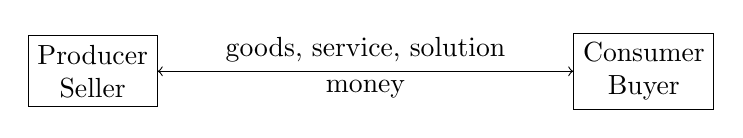
\begin{tikzpicture}
\node[draw, align=center] (p) at (0,0) {Producer\\Seller};
\node[draw, align=center] (c) at (7,0) {Consumer\\Buyer};
\draw[->] (p) -- node[above] {goods, service, solution} (c);
\draw[->] (c) -- node[below] {money} (p);
\end{tikzpicture}
\end{figure}

This small diagram is only a transcript-derived reconstruction, but it captures the lecture's first durable abstraction: value travels one way, money the other, and the question is which side of that exchange we mean to inhabit.

Once this distinction is in place, the speaker rapidly appends a second layer of discipline: fall in love with people, sales, and numbers. The point is subtle. Producer logic by itself is too crude. One must also be able to work with human beings, move an offer through speech, and keep accurate numerical account. From there the beat widens again: make speed work in your favor, do not procrastinate, be a giver rather than a taker, and work with total effort even while admitting that one person alone is not omnipotent. The lecture has not become a theorem, but it has become a system.

\section{Tech, Exits, and Speed to Market}

The next interview gives the first industry-specific sharpening of the earlier abstraction. We move from a general producer/seller distinction to a startup account of competition. The speaker says he grew up in the tech business, ran two companies for about ten years, and sold both for eight figures. The host then asks not merely about outcome but about entry: how does one break into tech in 2024?

The answer is built around speed. In the lecture's own phrasing, an idea today can be matched tomorrow. That means the relevant interval is the time between conception and market execution. The shorter that interval, the more likely it is that the originator captures the opportunity before imitation closes the gap. In that spirit we may summarize the logic schematically as follows:
\begin{equation}
\Delta t_{\mathrm{idea}\to\mathrm{market}} \downarrow
\quad \Longrightarrow \quad
\text{imitation risk before capture} \downarrow .
\end{equation}
This is not a measured law. It is a narrated rule of startup timing.

Two further supports are then added. First, great people: smart, committed people willing to live inside the 24/7 demands of a startup. Second, capitalization: not just money, but \emph{smart money}. The speaker's claim is that in tech it is not enough to have fuel; one wants fuel that carries judgment, network, and discipline with it. The industry recommendation at the end of the beat is blunt: tech, and more specifically AI, because software is where the world is visibly changing.

The host's recap compresses the lesson without flattening it. Speed matters, but the deeper enabler is human quality. The lecture is beginning to braid timing and people together.

\section{Freedom, Complaint, and the Solution Habit}

The immigrant-founder beat changes the emotional register while keeping the commercial thread intact. The speaker says she came to the United States with \text{\$}78 in cash, did not speak English, and now makes about \text{\$}2 million annually:
\begin{equation}
M_0 = \text{\$}78,
\qquad
I_{\mathrm{annual}} \approx \text{\$}2\,\mathrm{M}.
\end{equation}

\begin{remark}
We should not force these two numbers into a false growth law. The first is an initial stock of cash; the second is a later annual flow. The lecture's point is directional and narrative, not actuarial.
\end{remark}

What matters here is not simply the move from a small number to a large one. The speaker says the favorite part of being a business owner in the United States is freedom. Money is therefore not treated as the terminal object. It is treated as a means by which poverty does not get repeated onto one's children and oneself.

The next question is one of the lecture's finest because it replaces biography with shared trait: what do successful people have in common? The answer is not genius, pedigree, or perfect conditions. It is that they do not complain. They stay on the side of solution. They ask, ``What can I do better?'' rather than sinking into self-pity.

The final advice in this beat is equally structural. Do not take instruction from people who do not possess the thing you want. Ignore noise. Become obsessed with the craft itself. In the speaker's example, even a strange or easily mocked business can work if the operator becomes preoccupied with mastery rather than with social permission. The host's recap is sharp: the anti-entitlement habit matters because work, not complaint, is the variable one can actually control.

\section{Gross, Net, and Accountability}

We now reach the lecture's most overtly operational segment. A young entrepreneur reports a short but intense business history, a main marketing agency feeding other companies in an ecosystem, and a first full year at \text{\$}5.5 million gross but \text{\$}2.4 million net:
\begin{align}
G &= \text{\$}5.5\,\mathrm{M},\\
N &= \text{\$}2.4\,\mathrm{M},\\
N &= G - K.
\end{align}
Here \(K\) stands for the aggregate subtraction between the top line and the retained result: cost, operating expense, leak, and all the rest. The speaker's own emphasis is decisive: ``net'' is the figure that truly matters.

\paragraph{Worked Example.}
From the transcript's reported numbers we can do a careful piece of arithmetic, while remembering that we are not reconstructing audited accounts.
\begin{enumerate}
\item Start with the spoken top line and retained result:
\[
G=\text{\$}5.5\,\mathrm{M},
\qquad
N=\text{\$}2.4\,\mathrm{M}.
\]
\item Infer the residual cost bucket:
\[
K = G-N = \text{\$}3.1\,\mathrm{M}.
\]
\item Compute the retained fraction of gross:
\[
\frac{N}{G} \approx \frac{2.4}{5.5} \approx 0.436.
\]
\item Thus about \(43.6\%\) of the reported gross survives into the figure the speaker values, while the remaining \(56.4\%\) is consumed by the machinery of operating at that scale.
\end{enumerate}
The lecture's lesson is simple: scale without retention is a weaker achievement than many spectators suppose.

The same speaker then narrates repeated resets: an early clothing store and barbershop, collapse under bad partnership conditions, restart through phone sales, losses in real estate, and then a move into insurance because it appeared to be an ``unlimited earning potential vehicle.'' The precise word ``unlimited'' should be handled cautiously; what the lecture clearly means is that the compensation structure was not visibly capped in the way earlier experiments had been.

\subsection{Question \& Answer}

\paragraph{Question.} What keeps people broke?

\paragraph{Answer.} The answer is not that bad things happen. The sharper answer is that people fail to convert bad things into managed problems. The speaker's memorable formula is that an event may not be your fault, but it is still your problem. Once the lecture says this, it immediately names concrete failure points: money management, time management, and the refusal to prospect.

This gives us a second operational chain:
\begin{equation}
P_t \uparrow \Rightarrow L_t \uparrow \Rightarrow S_t \uparrow,
\end{equation}
where \(P_t\) is prospecting effort, \(L_t\) the stock of active relationships or conversations, and \(S_t\) realized sales. The speaker insists that talent in selling is useless if one never enters the prospecting phase. In his most pointed example, 8 a.m.\ matters because that is when lawful prospecting may begin. Delay is therefore not morally bad in the abstract; it is economically bad because it postpones contact.

A third chain is psychological but still operational:
\begin{equation}
B_t \uparrow \Rightarrow W_t \uparrow \Rightarrow P_t \uparrow,
\end{equation}
where \(B_t\) denotes belief in oneself and \(W_t\) work intensity. Again, this is not psychometrics. It is the lecture's way of ordering cause: weak belief leads to weak effort, weak effort to weak prospecting, and weak prospecting to poor sales.

The host's recap after this interview is one of the cleanest in the lecture. He keeps the quantitative boast in place but extracts the true rule: whether or not the original injury was one's fault, one must still solve it. That is the accountability doctrine.

\section{Cash Flow and Real Estate Compounding}

The mansion interview shifts us from earning to deployment. An orthodontist says he has made multiple millions, pushed money into real estate and shopping centers, and now explains what he means by creating wealth in property. The conceptual move here is important. Wealth is no longer treated as the direct consumption of a large house. It is treated as a reinvestment process.

\subsection{Question \& Answer}

\paragraph{Question.} How do we create wealth in real estate without beginning with a ton of money?

\paragraph{Answer.} The speaker's answer is recursive. We first build a core practice that grows. That practice produces cash flow. We then use that cash flow to acquire shopping centers or medical buildings. Those assets themselves produce cash flow. The next round begins from a higher base.

In cautious notation, the lecture's mechanism can be summarized as
\begin{align}
C_{t+1} &= C_t^{\mathrm{practice}} + C_t^{\mathrm{asset}},\\
A_{t+1} &= A_t + \Delta A(C_t).
\end{align}
The first line says that next-period deployable cash is the sum of cash from the core business and cash from already-acquired assets. The second says that the asset stock grows by whatever purchases current cash flow can support.

\begin{figure}[h]
\centering
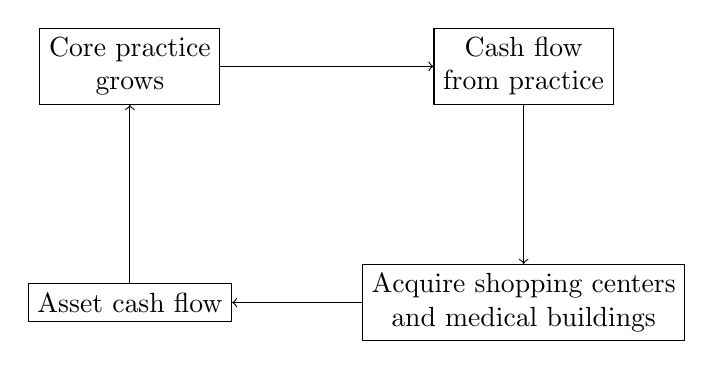
\begin{tikzpicture}
\node[draw, align=center] (practice) at (0,0) {Core practice\\grows};
\node[draw, align=center] (cash) at (5,0) {Cash flow\\from practice};
\node[draw, align=center] (buy) at (5,-3) {Acquire shopping centers\\and medical buildings};
\node[draw, align=center] (asset) at (0,-3) {Asset cash flow};
\draw[->] (practice) -- (cash);
\draw[->] (cash) -- (buy);
\draw[->] (buy) -- (asset);
\draw[->] (asset) -- (practice);
\end{tikzpicture}
\end{figure}

This loop is a transcript-derived reconstruction, but it is the clearest mechanism in the lecture. We do not need a complicated return model to see the point. The business throws off cash; cash buys assets; assets throw off more cash; the process repeats.

The speaker then adds two correctives. First, a professional degree may matter if one wants access to higher-barrier core businesses such as medicine or law. Second, even in property, deal flow is social. He says the last two deals happened because he got directly in front of the owner and was liked. Thus the reinvestment loop is not purely financial. It rests on both cash generation and human access.

\section{Feeding the Business and Selling at Scale}

The private-jet capstone moves the lecture to its highest scale and its most mature operating philosophy. We hear of thirty years in business, tens of millions in yearly earnings, \text{\$}100 million exits, and a best year at
\begin{equation}
R_{2023}=\text{\$}752\,\mathrm{M}.
\end{equation}
But once again the number itself is not the lecture's terminus. It is a way of licensing the next set of rules.

The first is a rule about learning: ask questions. The speaker is almost offended by the idea that someone would be in a room with a superior operator and remain silent. Curiosity is not presented as decoration. It is presented as an accelerant.

\subsection{Question \& Answer}

\paragraph{Question.} What is the best financial advice for building a sustainable business?

\paragraph{Answer.} Two answers are layered together. The first is to feed the business rather than starve it. If margins are thin and the model takes time, one must still keep the company resourced long enough for its scale to matter. The second is the three-legged stool: a decision must work for the customer, the worker side, and the company itself.

We can formalize that second test schematically:
\begin{equation}
D\ \text{admissible}
\iff
E_{\mathrm{cust}}(D)\ge 0,\ 
E_{\mathrm{team}}(D)\ge 0,\ 
E_{\mathrm{firm}}(D)\ge 0.
\end{equation}
Here \(D\) is a business decision, and the \(E\)'s are the effects of that decision on the three constituencies. This is not how the speaker phrases it, but it is faithful to the structure: if one leg collapses, the stool is unstable.

\begin{figure}[h]
\centering
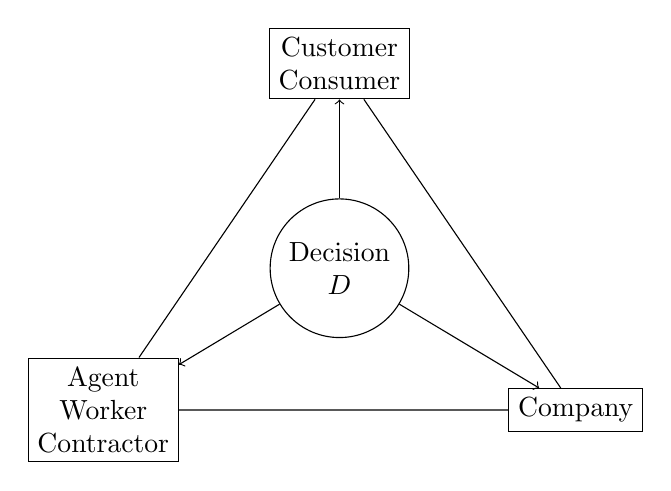
\begin{tikzpicture}
\node[draw, align=center] (top) at (0,2.6) {Customer\\Consumer};
\node[draw, align=center] (left) at (-3,-1.8) {Agent\\Worker\\Contractor};
\node[draw, align=center] (right) at (3,-1.8) {Company};
\node[draw, circle, align=center] (center) at (0,0) {Decision\\\(D\)};
\draw[->] (center) -- (top);
\draw[->] (center) -- (left);
\draw[->] (center) -- (right);
\draw (top) -- (left) -- (right) -- (top);
\end{tikzpicture}
\end{figure}

What follows is the lecture's most subtle distinction between visible richness and structural freedom. The speaker says many people enter business to get rich immediately. He entered business to get free, believing that wealth would come later. This is not a pious slogan. It is a capital-withdrawal rule. If one extracts too early, one may look rich and remain weak. If one feeds the business, one may look poorer and become stronger.

From here the lecture slides naturally into sales. Most people struggle, the speaker says, because they do not believe in themselves, and that weak belief lowers effort. His own account of sales is aggressively behavioral: make more calls, worry less about being judged, refuse to stop at the first no, and understand that the field is less competitive than it appears because many people will not work.

Schematically, the lecture's sales doctrine can be written as
\begin{equation}
B_t \uparrow \Rightarrow W_t \uparrow \Rightarrow P_t \uparrow \Rightarrow L_t \uparrow \Rightarrow S_t \uparrow.
\end{equation}
Belief raises work, work raises prospecting, prospecting raises the number of live relationships, and relationships make sales possible. The important point is that the causal chain begins earlier than closing technique.

This is also where the lecture's other maxims settle into place: the first rule of business is to stay in business; if people around us act like anchors, we do not let them pull us under; and the correct response to the accusation ``you think you're better than us'' is not superiority but asymmetry of appetite. One simply wants more.

\section{Summary}

The lecture begins with spectacle but is strongest when it becomes structural. Its recurring distinctions are the real content: producer versus consumer, buyer versus seller, gross versus net, complaint versus solution, rich versus free. From those distinctions we obtain a sequence of practical update rules. Speed matters in tech because imitation is fast. Cash flow matters in real estate because assets can be bought from it and then add to it. Prospecting matters in sales because talent cannot monetize without contact. Patience matters in business because the company must be fed before it can carry us.

What makes the lecture worth preserving is that it never leaves the level of mere inspiration. Even its motivational lines are attached to mechanisms. The strongest operators in the transcript think in flows, positions, constraints, and repeated loops. That is as close as this lecture comes to a blackboard, and it is close enough to deserve careful notes.